\section{Módulo de Apresentação}
\label{sec:modulo_apresentacao}

	Após o marcador ser reconhecido e identificado, o Módulo de Apresentação fica responsável por
	apresentar ao usuário todos os recursos disponíveis do dispositivo selecionado. São aceitos os
	mesmos recursos compatíveis com a Hydra: câmera, \textit{mouse}, teclado ou tela. Os recursos são
	visualizados através de um objeto virtual, ao qual é apresentado na tela. Este é representado
	através de um retângulo onde é exibido o nome do dispositivo e os recursos por ele
	disponibilizados. Na figura \ref{fig:objeto_virtual}, podemos observar um caso onde temos o 
	dispositivo iMacDevice que disponibiliza os seus recursos de câmera,~\textit{mouse}, tela e teclado.

	
	\begin{figure}[htb]
		\centering 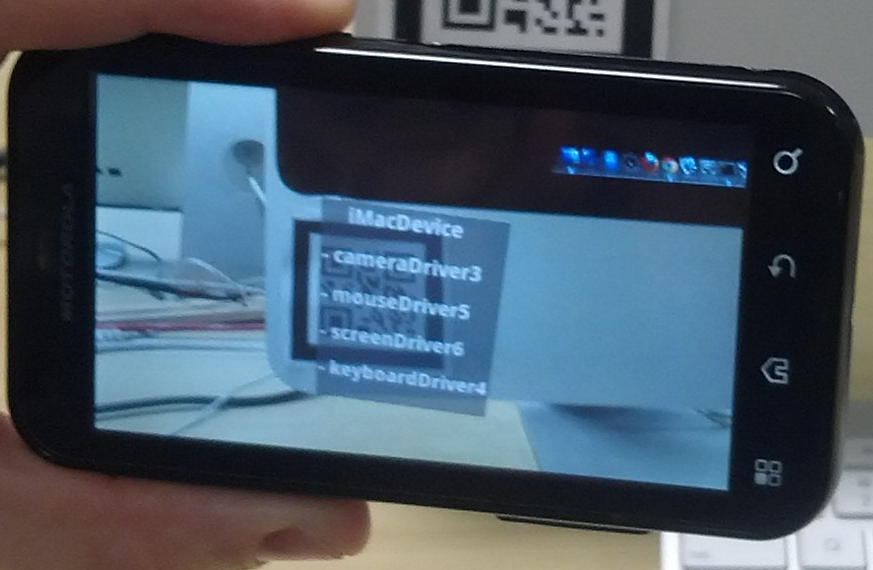
\includegraphics[scale=0.3]{figuras/cap4/objeto_virtual.png}
		\caption{\textit{Objeto virtual.}}
		\label{fig:objeto_virtual} 
	\end{figure}
	
	Para interagir com o dispositivo basta ao usuário tocar a tela sobre o objeto que o representa.
	Desta forma é exibida uma nova tela onde é possível controlar o uso dos recursos do dispositivo.
	Possibilitando ao usuário selecionar o redirecionamento ou liberação conforme desejado. A 
	figura~\ref{fig:listagem_recursos} mostra o detalhamento dos recursos disponíveis ao usuário no 
	dispositivo. Os recursos de teclado e \textit{mouse} já estão sendo redirecionados para a Hydra, 
	enquanto os demais estão disponíveis para serem utilizados pela mesma.
	
	
	\begin{figure}[htb]
		\centering 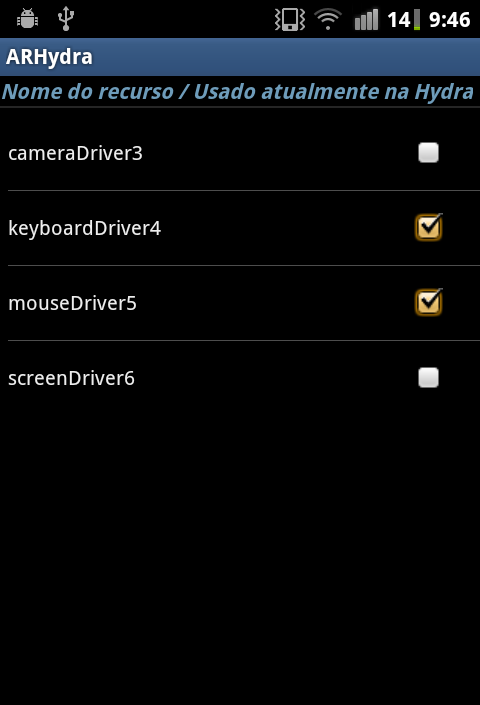
\includegraphics[scale=0.35]{figuras/cap4/listagem_recursos.png}
		\caption{\textit{Listagem dos recursos.}}
		\label{fig:listagem_recursos} 
	\end{figure}
	
	O \textit{framework} DroidAR \cite{droidar} foi utilizado para facilitar a renderização dos objetos 
	na tela. Para o gerenciamento desses objetos virtuais fez-se necessário a criação de uma classe 
	responsável pela criação, reposicionamento e deleção desses objetos. Essa classe recebe informações
	dos Módulos de Reconhecimento e Decodificação para determinar a ação a ser executada. A interação
	desse controle com os demais módulos é apresentado na figura~\ref{fig:condicoes_objeto}.

	\begin{figure}[htb]
		\centering 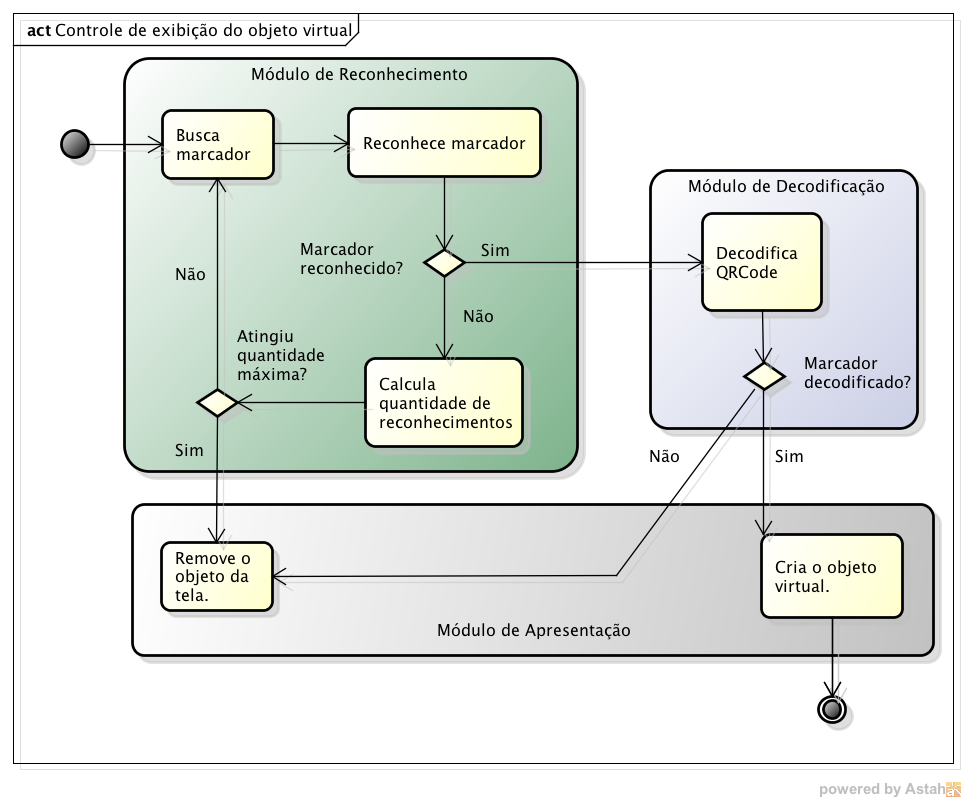
\includegraphics[scale=0.55]{figuras/cap4/condicoes_objeto.png}
		\caption{\textit{Condições para visualização do objeto virtual.}}
		\label{fig:condicoes_objeto} 
	\end{figure}

	Desta maneira, o controle de exibição dos objetos virtuais possibilita uma correta visualização
	dos recursos disponíveis pelos dispositivos. De modo que somente os recursos de um dispositivo
	sejam apresentados por vez.
	
